% Created 2025-05-07 Wed 18:33
% Intended LaTeX compiler: pdflatex
\documentclass[11pt]{article}
\usepackage[utf8]{inputenc}
\usepackage[T1]{fontenc}
\usepackage{graphicx}
\usepackage{longtable}
\usepackage{wrapfig}
\usepackage{rotating}
\usepackage[normalem]{ulem}
\usepackage{amsmath}
\usepackage{amssymb}
\usepackage{capt-of}
\usepackage{hyperref}
\date{\today}
\title{Report 1}
\hypersetup{
 pdfauthor={maikito},
 pdftitle={Report 1},
 pdfkeywords={},
 pdfsubject={},
 pdfcreator={Emacs 29.3 (Org mode 9.7.19)}, 
 pdflang={English}}
\usepackage{biblatex}

\begin{document}

\maketitle
\tableofcontents

\section{Research question and hypotheses}
\label{sec:org5f7e195}
Does the brain keep track of the values associated with all possible policies, or only the currently exploited one? What drives our decision-making process as value computation becomes less tractable/more uncertain? We hypothesize that, as task complexity and uncertainty increase, the decision-making process goes from: value-comparison driven, to value-comparison-to-threshold driven, to ``consequence'' driven. By consequence, we mean the change in mean reward between trials (\(\Delta \bar{R}\)). A ``consequence'' driven agent seeks high reward states, but does not compute value.
To test the above hypotheses, we developed a novel perceptual decision-making task.
\section{Task}
\label{sec:orgec8ef80}
\subsection{Stimuli generation}
\label{sec:org0da1f59}
The mean of the stimuli in Trial 1, \(m\), has bounds: \(\\ ( |g| + \frac{\max d}{2} , 1 - |g| - \frac{\max d}{2} )\) \\
There are 10 possible values of m for each g. These values are linearly spaced between the lower and upper bounds and are sampled at random before each episode. These bounds ensure the minimum and maximum stimuli values are 0 and 1, respectively. \\

The stimuli heights are then computed as follows: \\
Trial 1 stimuli heights: \(m \pm \frac{d}{2} \\\)
Trial 2 stimuli heights: \(\begin{cases}
                                                m \pm \frac{d}{2} + g \text{ if chose small}  \\
                                                m \pm \frac{d}{2} - g \text{ if chose big}
                                                \end{cases}
                                                \\\)


Difficulty, d, determines the magnitude of the difference in stimuli heights in an episode. A single value of d \(\in\) \{0.05, 0.2, 0.35\} is randomly chosen before each episode. d is constant within an episode.  \\
Gain, g, determines the magnitude and sign of the consequence of the Trial 1 choice. Each block consists of 30 episodes and has a single value of g. In total there are 4 blocks, one for each value of g \(\in\) \{-0.3, 0, 0.1, 0.3\}. The order of these blocks is random. \\
\subsection{Determining Gain (g) and Difficulty (d)}
\label{sec:org87a5fba}
Gain and difficulty are two of the most important task parameters. They determine the magnitude (and sign) of consequence as well as the magnitude of the difference between stimuli presented in a given trial. These parameters determine the optimal strategy.
Proper selection of g and d should allow us to determine whether participants' decisions are primarily determined by 1) value comparison, 2) comparison to threshold, or 3) ``consequence''.
\subsubsection{Original values}
\label{sec:orgf6e6c91}
The previous g was 0.3 for Horizon 1. The previous d values were: [0.01, 0.05, 0.1, 0.15, 0.2].

These values of g and d meant that Small-Big was always the optimal action sequence/policy in Horizon 1. In other words, giving up 0.2 units of reward in trial 1 was always worth it since the mean reward of the stimuli would increase by 0.3.
\subsubsection{Updated values}
\label{sec:orgbae44be}
More values of g, along with appropriate values of d, are required in order to determine how humans decide in the consequential task. I propose four values of g:

\begin{table}[htbp]
\label{Table 1}
\centering
\begin{tabular}{llrl}
\hline
Condition & G & g & \(\pi\)*\\
\hline
A & G < 0 & -0.3 & Big-big\\
B & G = 0 & 0 & Big-big\\
C & G = c & 0.1 & Small-big \textasciitilde{} Big-big\\
D & G > c & 0.3 & Small-big\\
\end{tabular}
\end{table}

I propose the following d values: [0.05, 0.2, 0.35]

The data below is the output from a Python script in which I computed the cumulative reward for the two possible action sequences (small-big \& big-big) and for all combinations of g and d:

\phantomsection
\label{}
\begin{verbatim}
g:  [-0.3, 0, 0.1, 0.3]
difficulty:  [0.05, 0.2, 0.35]


(cum reward small-big, cum reward big-big)
             0.05         0.2         0.35
-0.3  (0.7, 1.35)  (0.7, 1.5)  (0.7, 1.65)
0     (1.0, 1.05)  (1.0, 1.2)  (1.0, 1.35)
0.1   (1.1, 0.95)  (1.1, 1.1)  (1.1, 1.25)
0.3   (1.3, 0.75)  (1.3, 0.9)  (1.3, 1.05) 

(cum reward small-big) - (sum reward big-big)
      0.05  0.2  0.35
-0.3 -0.65 -0.8 -0.95
0    -0.05 -0.2 -0.35
0.1   0.15  0.0 -0.15
0.3   0.55  0.4  0.25
\end{verbatim}

The second ``table'' above shows shows the difference in cumulative reward, for all g and d, between the Small-Big and Big-Big action sequences. These values of g and d yield the optimal strategies outlined in Table 1. For these proposed values, the optimal policy is Big-Big for g=-0.3 and g=0. For g=0.1, Small-Big and Big-big yield identical cumulative reward.  The optimal strategy, in this case, is Small-Big when d is large and Big-Big when d is small. Small-Big and Big-Big yield identical cumulative reward when d is 0.2 (the intermediate value). Finally, the optimal strategy is Small-Big when g=0.3.
\subsection{Instructions for participants}
\label{sec:org31aae5e}
\begin{center}
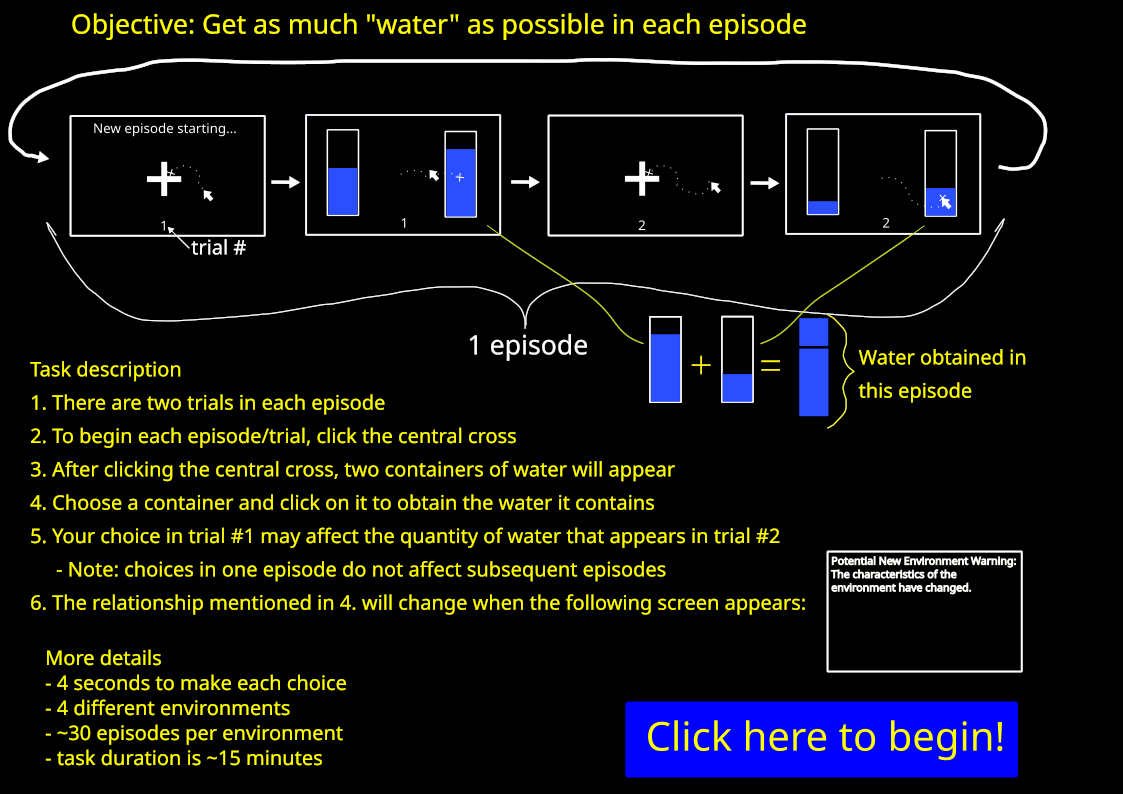
\includegraphics[width=.9\linewidth]{./img/instructions.png}
\end{center}
\subsection{Differences between Horizon 1 v1 \& Horizon 1 v2}
\label{sec:orgc829446}
Table 2 shows most of the important differences between version 1 and version 2 of the task.
\begin{table}[htbp]
\label{Table 2}
\centering
\begin{tabular}{lll}
attribute & v1 & v2\\
\hline
g & 0.3 & \{-0.3, 0, 0.1, 0.3\}\\
d & \{0.01, 0.05, 0.1, 0.15, 0.2\} & \{0.05, 0.2, 0.35\}\\
\(\pi\)* & Small-Big & g \& d dependent\\
fixation timeout & skip trial & progresses trial\\
stimuli selection & mouse hover & mouse click\\
\end{tabular}
\end{table}
\subsection{Uncertainty in the Consequential task}
\label{sec:org091c3ce}
\subsubsection{Sources of uncertainty}
\label{sec:org577c035}
\begin{enumerate}
\item Visual discrimination/perceptual uncertainty
\label{sec:orgf611678}
At least two kinds of uncertainty result from visual perception in the Consequential task.
\begin{enumerate}
\item For the smallest d, it can be difficult to determine which stimulus is larger.
\item It can be difficult to visualize and quantify the sum of the two chosen stimuli in an episode.
\begin{itemize}
\item This makes value computation more difficult, which, consequently, makes value comparison between policies more difficult.
\end{itemize}
\end{enumerate}
\item Lack of performance feedback
\label{sec:orgffcad0d}
The lack of performance feedback means participants never know if they are employing the optimal strategy.
\item Lack of knowledge regarding which aspects of the stimuli are important
\label{sec:orgf028adc}
Participants don't know if the relative height of the stimuli is the only important attribute of the stimuli. Participants may expore other stimuli attributes such as position on screen (i.e., left/right) or order of presentation on the screen (i.e. first/second). It is also conceivable that participants may check whether g is a function of m, d, or reaction time.
\end{enumerate}
\subsubsection{Modulating uncertainty}
\label{sec:org2767359}
Modulating uncertainty is important since one of our primary hypotheses is that the decision process shifts away from value-comparison as uncertainty increases. Below I propose two changes to the current Horizon 1 v2 task which would yield four versions of the task.
\begin{table}[htbp]
\label{Table 3}
\centering
\begin{tabular}{llll}
task version & uncertainty & g & value feedback\\
\hline
A & Low & constant & yes\\
B & Medium & stochastic & yes\\
C & Medium & constant & no\\
D & High & stochastic & no\\
\end{tabular}
\end{table}
Task version C corresponds to the current version.
\begin{enumerate}
\item Stochastic g (increases uncertainty)
\label{sec:org814998a}
Rather than g being held constant in each block, g could be sampled before each episode from a distribution with mean g. This would make value computation more difficult but, crucially, would not affect the optimal policy.
\item Value feedback (decreases uncertainty)
\label{sec:orga882870}
In the present version of the task, the participants must visualize and quantify the sum of the two selected stimuli in their minds. They must also remember this value to then compare it with the approximated values of other policies. I propose making a version of the task with value feedback in which the sum of the selected stimuli is presented at the end of each episode along with a numerical representation of this sum. This would remove all uncertainty in value computation of the exploited policy.
\end{enumerate}
\subsection{Open questions regarding the task}
\label{sec:org926c39e}
\begin{enumerate}
\item Since we are primarily interested in value computation in the present project, should we try to eliminate sources of uncertainty that are less related to value computation? For example, should I include ``Note: the only relevant attribute of the containers is the amount of water they contain. Other aspects of the containers (e.g., whether the container is on the left or right side of the screen) are irrelevant.'' in the instructions?
\item Should there be a monetary performance bonus for participants?
\begin{itemize}
\item This would increase motivation. I could, at least, provide some performance-related feedback at the end of the experiment. I could also state in the instructions that they will receive a ``score'' at the end of the experiment. This may be a way of increasing motivation in lieu of a monetary bonus.
\item The nature of this bonus/feedback is important since participants will likely be more explorative if they only care about finding the optimal policy. If, however, participants know there is a monetary bonus or score proportional to the total amount of reward/``water'' acquired in the experiment, then they may be more likely to continue exploiting suboptimal strategies if their associated values are above a certain threshold (i.e., foraging).
\end{itemize}
\item The current version of the task (task version C) takes roughly 15 minutes to complete. Should I employ a repeated measures design (i.e. every participant performs all versions of the task), or should I use an independent measures experimental design?
\begin{itemize}
\item I'm leaning towards independent measures. I think it's more likely that participants will pay full attention and perform if the experiment only last 15 minutes. We can add a repeated measures group later if desired.
\item One argument in favor of a repeated measures design is seeing how exposure to a a low uncertainty version of the task (e.g. with value feedback) may affect performance in subsequent versions of the task (e.g. without value feedback).
\end{itemize}
\end{enumerate}
\section{Cognitive models}
\label{sec:orge5d862f}
I propose to investigate two types of cognitive models (i.e., agents): value-comparison driven \& consequence driven. I propose to implement to versions of each type of model: option comparison \& comparison to threshold.
\subsection{Value comparison}
\label{sec:org64aa285}
For the value-comparison case, I propose to use a classical model-free Q-learning algorithm with the following q-table:
\begin{center}
\begin{tabular}{|l|l|l|}
\hline
state & action: small & action: big\\
\hline
trial 1, small d & q1 & q2\\
trial 1, large d & q3 & q4\\
trial 2, large \(\bar{R}\) & q5 & q6\\
trial 2, small \(\bar{R}\) & q7 & q8\\
\hline
\end{tabular}
\end{center}
The update rule would be:
\begin{equation}
Q(S, A) \gets Q(S, A) + \alpha (R + \gamma \max_a Q(S', A') - Q(S, A))
\end{equation}
The input to the choice rule for a given state will be the q values associated with that state (e.g., decisions in the ``trial 1, small d'' state will be determined by q1 and q2).
\subsection{Value comparison to threshold}
\label{sec:org2e5561c}
The value comparison to threshold agent's actions are driven by the comparison of the state-action values of the currently exploited strategy to a threshold, sometimes referred to as a ``satisfaction'' threshold. This decision-making strategy is compelling since we often settle for satisfactory action sequences rather than searching for truly optimal ones.
The q-table for this agent is the same as in the value comparison case.
The update rule is also identical.
We will choice rule similar to the value comparison agent, however, the input to the choice rule function will be the q-value associated with the currently expoited strategy, and a ``satistfaction'' threshold, \(\rho\). Decisions in the ``trial 1, small d'' state will be determined by the q-value corresponding to the currently exploited strategy (i.e., the q-value corresponding to the action taken in the previous episode) and \(\rho\).
\subsection{Consequence comparison}
\label{sec:org7e2102a}
The consequence-driven agent does not compute value. Instead, this agent seeks high-reward (\(\Delta\bar{R}\)) states.
The states and actions are the same as the previous cases, the ``q-table'', however is updated differently. Since q is typically used to refer to value, I will call the updated values consequence values, or c-values. C-values are updated based on the reward obtained in the current state as well as the change in mean reward between the current and subsequent states.
The update rule is the following:
\begin{equation}
C(S, A) \gets C(S, A) + \alpha (R + \gamma (\bar{R'} - \bar{R}) - C(S, A))
\end{equation}
Is is also conceivable that paricipants focus entirely on \(\Delta\bar{R}\), and ignore reward acquired in the current state. For this reason, I propose to introduce one additional tunable parameter:
\begin{equation}
C(S, A) \gets C(S, A) + \alpha (\beta_1 R + \beta_2 (\bar{R'} - \bar{R}) - C(S, A))
\end{equation}
\subsection{Consequence comparison to threshold}
\label{sec:orge48f254}
The consequence analog of value comparison to threshold.
\subsection{Drift diffusion model choice rule}
\label{sec:org61d8a30}
We will use a drift diffusion model as the choice rule for all agents. This will enable us to fit participants' reaction times (RT). The input to the DDM is different for each model, but the number of tunable parameters is the same, thus the addition of the DDM does not affect the complexity of the models relative to one another. To begin, I propose to use a constant scaler for the drift rate, \(v\), constant diffusion boundaries, and a non-biased starting point, \(z\). This reduces the complexity of the model. We may choose to fit these parameters if the simple version of the model results in a poor fit.
\subsection{Model fitting \& cross validation}
\label{sec:org3077a84}
I propose to fit the reinforcement learning parameters and the DDM parameters simultaneously via hierarchical Bayesian parameter estimation. Hierarchical Bayesian parameter estimation is convenient in that it provides both individual and group-level parameters.
After model fitting, I propose to use leave-one-out cross validation to determine the goodness-of-fit of each cognitive model.
\end{document}
